\begin{comment}
Ergebnisse der Arbeit: was wurde erreicht, was wurde nicht erreicht, Ursachen.
Dieser Abschnitt richtet sich an den speziell für das entsprechende Fachgebiet
interessierten Ingenieur. Er soll es ihm ermöglichen, die für die Problemlösung
gemachten Überlegungen zu verstehen und nachzuvollziehen. Theoretische
Grundlagen sind nur so weit auszuarbeiten, als dies für die Lösung der Aufgabe
nötig ist (keine Lehrbücher schreiben). Die Erkenntnisse aus den theoretischen
Untersuchungen sind wenn immer möglich direkt mit der Problemlösung zu
verknüpfen.

Schlussfolgerungen, Bewertung der Ergebnisse.
Die Schlussfolgerungen bilden zusammen mit der Zusammenfassung die
wichtigsten Abschnitte eines Berichts und sollen daher am sorgfältigsten
ausgearbeitet sein. Die Schlussfolgerungen enthalten eine Zusammenfassung
und Beurteilung der Resultate (Vergleich mit anderen Lösungen, was wurde
erreicht, was nicht, was bleibt noch zu tun, was würde man nun anders tun). In
den Schlussfolgerungen soll auch ein Ausblick auf das weitere Vorgehen bzw.
auf die Bedeutung der erreichten Ergebnisse gegeben werden.

Installationsanleitung vorhanden (inklusive verwendete Entwicklungsumgebung und Werkzeuge), Test-Logs dokumentiert (bei Systemen mit User Interfaces: Dokumentation der Usability Tests)
\end{comment}

\chapter{Ergebnis}
\xxx

\xxx[Erwähnen dass Regelwerk-Feature abgelehnt wurde]

\begin{figure}[H]
	\centering
	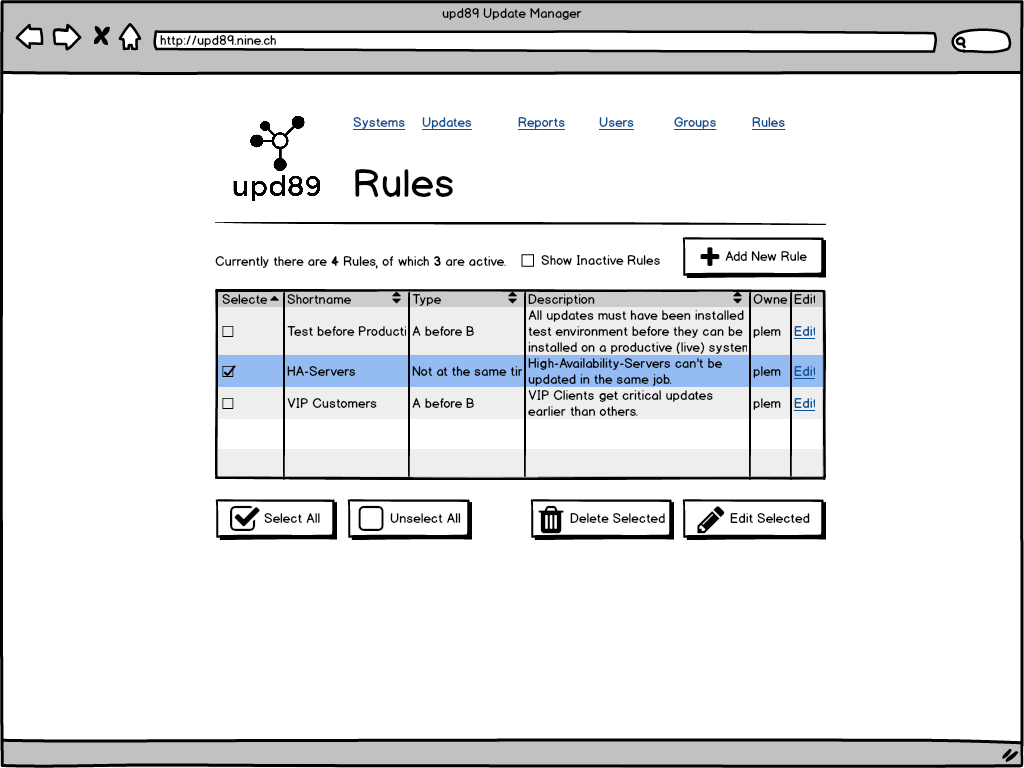
\includegraphics[width=\linewidth]{files/mockups/rules}
	\caption{Verworfenes Regelwerk-Feature}
	\label{fig:ergebnis:rules}
\end{figure}

\section{Schlussfolgerung}
\xxx

\section{Softwaredokumentation}
\xxx

